\section{Algebra, Geometry and Algorithms} 

\textbf{{Linear Algebra}} 
\normalsize
\begin{itemize}
    \item \textcolor{blue}{Algebra:} linear equations 
    \item \textcolor{blue}{Geometry:} sets defined by linear subsystems of equtions, affine subspaces, vectors, vector subspaces, ... 
    \item \textcolor{blue}{Algorithms:} Gaussian elimination
\end{itemize}
\begin{center}
\begin{tikzpicture}[scale=0.8]
 \definecolor{kOrange}{RGB}{250,130,20}
  \definecolor{kGreen}{RGB}{50,130,40} 

  % Geraden
  \draw[name path=g, thick, kOrange]  (-3,-1) -- (3,0.5)  node[right] {$g$};
  \draw[name path=h, thick, kGreen]   (-3,0.5)  -- (3,-1) node[right] {$h$};

  % Schnittpunkt
  \path[name intersections={of=g and h, by=S}];
  \fill[black] (S) circle (2.5pt) node[above=4pt] {$S$};
\end{tikzpicture}
\end{center}

\textbf{{Non-Linear Algebra}}
\normalsize
\begin{itemize}
    \item \textcolor{blue}{Algebra:} polynomial equations 
    \item \textcolor{blue}{Geometry:} Varieties (sets defined by systems of polynomial equations) 
    \item \textcolor{blue}{Algorithms:} Buchberger's algorithm (a far-reading generalization of Gaussian elimination), Gröbner bases
\end{itemize}

\begin{center}
\begin{tikzpicture}[scale=0.65, x=0.0125cm, y=-0.0125cm, line cap=round, line join=round] 
      \useasboundingbox (100,40) rectangle (790,445);

   \definecolor{kOrange}{RGB}{250,130,20}
  \definecolor{kGreen}{RGB}{50,130,40}

  % orang
  \draw[name path=orangeCurve, kOrange, line width=1pt, use Hobby shortcut]
    (135,95) .. (240,48) .. (370,100) .. (335,183) .. (258,212) ..
    (168,283) .. (138,339) .. (160,410) .. (250,440) .. (330,425) ..
    (435,290) .. (473,244) .. (560,178) .. (637,165) .. (780,154);

%   grün
  \draw[name path=greenCurve, kGreen, line width=1pt, use Hobby shortcut, closed]
    (185,97) .. (155,230) .. (300,370) .. (420,425) .. (500,360) ..
    (430,255) .. (290,265) .. (258,212) .. (270,115) .. (330,160) ..
    (400,235) .. (473,244) .. (610,195) .. (645,150) .. (600,80) ..
    (50,230) .. (100,120);

  \path [name intersections={of=orangeCurve and greenCurve, name=S, total=\t}];
      \fill[black, name intersections={of=orangeCurve and greenCurve, name=S, total=\tot}]
    \foreach \i in {1,...,\tot} { (S-\i) circle[radius=2.5pt] };
\end{tikzpicture}
\end{center} 

\textbf{{The more Technical Layer}} \\[0.3em]
Notation of ideal in a ring \\ 
\hspace*{0.5cm} $\rightarrow$ this notation is relevant for the above topics but also for construction of rings and fields \\
\hspace*{1.2cm} (the latter is used in coding theory and cryptography)  

\subsection{Polynomials and the Affine Space} 

Variables considered per default in algebra are \textit{formal variables (symbols)}. Formal means roughly placeholder for anything. There is no domain attached to this. 

Formal variables are used in \textit{formal expressions (symbolic expressions)}. 

\textbf{Note the difference to functions}: Symbolic expressions are just expressions, not functions. In particular, they \hspace*{5.2cm}don't have any domain or co-domain.  \\

In what follows, we consider $n$ formal variables ($n \in \mathbb{Z}_{>0}$) whose default names will be $x_1, \ldots, x_n$.  If $n=1$ it's cosumary to use $x$ and $y$. For $n = 3$ it's cosumary to use $x, y, z$. 

\begin{definition}[title = Definition 1.1.1] 
    Let $x = (x_1, \dots, x_n)$ be the vector of $n$ formal variables and $\alpha = (\alpha_1, \dots, \alpha_n) \in \mathbb{Z}_{\geq 0}^n$ a vector of $n$ non-negative integers. Then the expression 
    \[x^{\alpha} := x_1^{\alpha_1} \cdot \ldots \cdot x_n^{\alpha_n}\] 
    is called the \textit{monomial for the expotent vector $\alpha$}.  $\alpha_1 + \ldots + \alpha_n$ is called the \textit{(total) degree of the monomial $x^{\alpha}$}, denoted as $|\alpha|$. \\[0.3em] 
    Our \textit{coefficient domain} will be an arbitrary field which we denote by $k$ thoughout.
\end{definition}

\clearpage

\begin{example}
    Given: $x^{2, 3} = x_1^2 \cdot x_2^3 \text{ and } x^{3, 0} = x_1^3$ 
    \begin{center}
        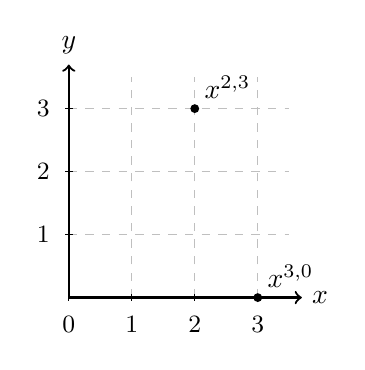
\begin{tikzpicture}[scale=0.8]
        \foreach \value in {1,2,3} {
          \draw[dashed, gray!50] (\value,0) -- (\value,3.5);
          \draw[dashed, gray!50] (0,\value) -- (3.5,\value);
        }
        \draw[->, thick] (0,0) -- (3.7,0) node[right] {$x$};
        \draw[->, thick] (0,0) -- (0,3.7) node[above] {$y$};
        \foreach \value in {0,1,2,3}
          \draw (\value,0.06) -- (\value,-0.06)
            node[below=2pt] {\small $\value$};
        \foreach \value in {1,2,3}
          \draw (0.06,\value) -- (-0.06,\value)
            node[left=2pt] {\small $\value$};
        \fill (2,3) circle (2pt) node[above right] {$x^{2,3}$};
        \fill (3,0) circle (2pt) node[above right] {$x^{3,0}$};
        \end{tikzpicture}
    \end{center}
\end{example}

You already know some fields: $\mathbb{Q}, \mathbb{R}, \mathbb{C}\mathbb{F}_p$ and $\mathbb{F}_{p^N}$ where $p$ is prime, $\mathbb{Q}[\sqrt{2}]$ 

\hspace*{0.5cm} $\rightarrow$ It's important to know some examples of them. 

\begin{definition}[title = Definition 1.1.2] 
    A \textit{polynomial in variables $x_1, \dots, x_n$} with coefficients in $k$ is a formal expression of the form 
    \begin{equation}
        f = \sum_\alpha c_\alpha x^\alpha, 
    \end{equation}
    where $\alpha$ runs over $\mathbb{Z}_{\geq 0}^n$ and $c_\alpha \neq 0$ for any finitely many choices of $k$. \\

    \hspace*{0.5cm}\textcolor{airforceblue}{\textit{(You must have seen polynomials in one variable before... surprise, surprise - life is not one-dimensional!)}}  \\

    $c_\alpha x^\alpha$ (when $c_\alpha \neq 0$) is called a \textit{term of degree} $|\alpha|$ of $f$. The \textit{(total) degree of $f$} is the maximum degree of the terms in $f$: \[deg f = \max\{|\alpha|: \alpha \in \mathbb{Z}_{\geq 0}^n, c_\alpha \neq 0\}\]
    
    The \textit{zero polynomial} $f =0$ has no terms and by this degree $-\infty$.  
    
    The \textit{set of all polynomials in $x_1, \dots, x_n$} with coefficients in $k$ is denoted by $k[x_1, \dots, x_n]$. \\
    
\begin{center}
  \textcolor{gray}{------------------------------------------- 06.10.2026 --------------------------------------------} \\[0.3em]
\end{center} 

    \textbf{Note:} Polynomials are formal expressions, not functions. \\[0.7em]
    Equality of two poynomials is defined through comparison of coefficients. \\[0.5em]
    We make $k[x_1, \dots, x_n]$ an algebraic stucture by introducing the basic operations, which are the addition and the multiplication. \\

    \textbf{Addition:} \[\sum_\alpha c_\alpha \cdot x^\alpha + \sum_\alpha d_\alpha \cdot x^\alpha := \sum_\alpha (c_\alpha + d_\alpha) \cdot x^\alpha\] 
    \textbf{Multiplication:} \[\left(\sum_\alpha c_\alpha \cdot x^\alpha\right) \left(\sum_\beta d_\beta \cdot x^\beta\right) := \sum_{\alpha, \beta} c_\alpha \cdot d_\beta \cdot x^{\alpha + \beta} = \sum_\gamma \left(\sum_{\alpha, \beta: \alpha + \beta = \gamma} c_\alpha \cdot d_\beta \right) \cdot x^\gamma\]
  \end{definition} 
\clearpage

\begin{remark}[title = Remark 1.1.3] 
    We can view $k$ as a subset of $k[x_1, \dots, x_n]$ and by this $k[x_1, \dots, x_n]$ contains $1\in k$ (The multiplecative identity). 

    It turns out that $(k[x_1, \dots, x_n], +, \cdot)$ is a unitary, commutative ring:   

    \begin{minipage}[t]{0.33\textwidth}
      \begin{align*}
          f+(h+g) &= (f+h)+g \\
          f+g &= g+f \\
          f + 0 & = f\\ 
          f + (-f) & = 0  
      \end{align*}
    \end{minipage}
    \begin{minipage}[t]{0.33\textwidth}
      \begin{align*}
          f \cdot (h \cdot g) &= (f \cdot h) \cdot g \\
          f \cdot g &= g \cdot f \\
          f \cdot 1 & = f\\ 
      \end{align*} 
    \end{minipage}
    \begin{minipage}[t]{0.33\textwidth}
      \begin{align*}
          (f + g) \cdot h & = f \cdot h + g \cdot h
      \end{align*}
    \end{minipage}

    This holds for all $f, g, h \in k[x_1, \dots, x_n]$. The $-f$ is the unique polynomial whose addition to $f$ gives 0.
\end{remark}

\begin{remark}[title = Remark 1.1.4]
    There are three basic choices of n:  
    \begin{center}
    \begin{tabular}{l|l|l}
      n = 1 & $x_1$ & x \\
      n = 2 & $x_1, x_2$ & x, y \\
      n = 3 & $x_1, x_2, x_3$ & x, y, z
    \end{tabular} 
  \end{center} 

    Later, a connection to geometry will be established. These three basic cases will get connected to line resp. plane and resp. 3-dim. space.
\end{remark}

\begin{definition}[title = Definition 1.1.5]
    In algebraic geometry, the space $k^n$ of all $n$-tuples with the coefficients in $k$ is called the \textit{$n$-dimentional affine space over the field $k$}.  
    
    From linear algebra we know, that $k^n$ is a $k$-vector space.  
\end{definition} 

\textbf{Fun Fact:} It's by far not the only space one can consider. Another very common and important space is the projective space. Actually, in the Elliptic Curve Cryptography (ECC), 
the elliptic curve is considered in the projective space.

\begin{definition}[title = Definition 1.1.6]
    We can evaluate $f = \sum_\alpha c_\alpha \cdot x^\alpha \in k[x_1, \dots, x_n]$ an a point $(a1, \dots, a_n) \in k^n$ of the affine space obtaining the value. 
    \[f(a1, \dots, a_n) = \sum_{\alpha = (\alpha_1, \dots, \alpha_n)} c_\alpha a_1^{\alpha_1} \cdots a_n^{\alpha_n}\]    
  
    This gives rise to to a function $k^n \to k$. This function is usually denoted again by $f$, even though $f \in k[x_1, \dots, x_n]$ and $f: k^n \to k$ is not the 
    same thing. In math, such a situation is called abuse of notation. 
    
    \hspace*{0.5cm}\textcolor{airforceblue}{\textit{I know it's not quite right, but I know what I'm doing}}
    
    Functions arising this way are called \textit{polynomial functions}.
\end{definition} 

\begin{remark}[title = Remark 1.1.7]
    In some fields, for example, in finite fields $k$, different polynomials in $k[x_1, \dots, x_n]$ may define the same polynomial function.
\end{remark} 

\clearpage
\begin{example}[title = Example]
Consider the finite field $\mathbb{F}_{2} = \{0, 1\}$ with 
\begin{tabular}{c| c c}
    + & 0 & 1 \\
    \hline
    0 & 0 & 1 \\
    1 & 1 & 0
\end{tabular}
and 
\begin{tabular}{c| c c}
    $\cdot$ & 0 & 1 \\
    \hline
    0 & 0 & 0 \\
    1 & 0 & 1
\end{tabular}

\vspace{0.3em} 

\begin{minipage}[t]{0.33\textwidth}
    $f = x^2 + x \in \mathbb{F}_2[x]$ \\
    $g = x^3 + x \in \mathbb{F}_2[x]$
\end{minipage}
\begin{minipage}[t]{0.33\textwidth}
  $f : \mathbb{F}_2 \to \mathbb{F}_2$

  \begin{tabular}{c |c}
    $a \in \mathbb{F}_2$ & $f(a) \in \mathbb{F}_2$ \\
    \hline
    0 & 0 \\
    0 & 0 
  \end{tabular}
\end{minipage}
\begin{minipage}[t]{0.33\textwidth}
  $g : \mathbb{F}_2 \to \mathbb{F}_2$

  \begin{tabular}{c |c}
    $a \in \mathbb{F}_2$ & $g(a) \in \mathbb{F}_2$ \\
    \hline
    0 & 0 \\
    0 & 0 
  \end{tabular}
\end{minipage}

So, both functions are the same, but the polynomials are different 
\end{example}

\textbf{Fun Fact:} Do we need $\mathbb{F}_2[x]$ for anything? \\
$\rightarrow$ Yes! Advanced Encryption Standard (AES) used the field $\mathbb{F}_{256}$, who construction requires taking a polynomial from $\mathbb{F}_2[x]$.  

\begin{theorem}[title =Theorem 1.1.8]
  Let the field $k$ be infinite. Then $f \in k[x_1, \dots, x_n]$ is a zero polynomial (all doefficients of $f$ are zero) if and only if $f: k^n \to k$ is a zero function.  
\end{theorem}
